%!TEX program = xelatex
%Template created by: Maciej Byczko
\documentclass[a4paper,12pt]{extarticle}  %typ dokumentu

\usepackage{geometry} %poprawienie marginesów
\usepackage{polski} %polskie znaki
\usepackage{graphicx} %grafiki
\usepackage{float} %poprawienie pozycji
\usepackage{fancyhdr} % header i footer
\usepackage{listings}
\usepackage{xcolor}
\usepackage{hyperref}
\graphicspath{{pictures/}}
\geometry{margin=0.7in}
\pagestyle{fancy}
\cfoot{Strona \thepage}
\rhead{Strona \thepage}
\lhead{\typdoc}
\setlength{\headheight}{15pt}

\title{\tytul \\ \small{\opis}}
\author{\tworcy}
\date{\data}

%-----------------------SEKCJA DANYCH----------------------------------
\def\tytul{Obsługa kamery USB} %<<< tytuł ćwiczenia
\def\nrcw{laboratoria 12} %<<< numer ćwiczenia
\def\data{\today} %<< data wykonania
\def\prowadzacy{Dr inż. Dominik Żelazny} %<<<prowadzący
\def\nrgrupy{D} %<<<numer grupy
\def\tworcy{Baraniecki Karol\\Byczko Maciej} %<<< autorzy
\def\zajinfo{PT 16:30 TP} %<<< informacje dotyczące zajęć
\def\typdoc{Sprawozdanie} %<<< typ dokumentu tj Sprawozdanie, zadania itp. {Matematyka dyskretna/Sprawozdanie z Miernictwa}
\def\opis{} %<<< opis który będzie umieszczony pod tytułem w Maketitle
%----------------------------------------------------------------------

\definecolor{backcolour}{rgb}{0.95,0.95,0.92}
\definecolor{AO}{rgb}{0,0.5,0}
\definecolor{ZeroBlue}{rgb}{0,0.28,0.73}
\definecolor{DarkRed}{rgb}{0.85,0.16,0.16}


\lstset{
basicstyle=\footnotesize,
breaklines=true,
language=Python,
numbers=left,
tabsize=2,
numberstyle=\tiny,
backgroundcolor=\color{backcolour},
breakatwhitespace=false,
showspaces=false,                
showstringspaces=false,
showtabs=false,
commentstyle=\color{gray},
keywordstyle=\color{ZeroBlue},
keepspaces=true,
% keywordstyle={[2]\color{DarkRed}},
% keywordstyle={[3]\color{ZeroBlue}},
}

\begin{document}
%-------------------------------------TABELA-DANYCH--------------------------------------------------
\begin{table}[H]
	\centering
	\resizebox{\textwidth}{!}{
		\begin{tabular}{|c|c|c|}\hline
			\begin{tabular}[c]{@{}c@{}}                     \tworcy     \end{tabular} &
			\begin{tabular}[c]{@{}c@{}}Prowadzący:\\        \prowadzacy \end{tabular} &
			\begin{tabular}[c]{@{}c@{}}Numer ćwiczenia\\    \nrcw       \end{tabular}          \\ \hline
			\begin{tabular}[c]{@{}c@{}}                     \zajinfo    \end{tabular} &
			\begin{tabular}[c]{@{}c@{}}Temat ćwiczenia:\\   \tytul      \end{tabular} & Ocena: \\ \hline
			\begin{tabular}[c]{@{}c@{}}Grupa:\\          \nrgrupy    \end{tabular}    &
			\begin{tabular}[c]{@{}c@{}}Data wykonania:\\    \data       \end{tabular} &        \\ \hline
		\end{tabular}}
\end{table}
%----------------------------------------------------------------------------------------------------
\section{Zagadnienia do opracowania}
\begin{enumerate}
	\item Zasada działania skanera płaskiego - rodzaj skanera obrazu.

	      Pokrywa skanera jest ruchoma, pod nią znajduje się szyba. Aby dokonać skanowania, kładzie się skanowaną kartkę na szybę skanowaną stroną do spodu. W trakcie pracy skanera pod szybą przesuwa się zespół lampa-lustro.

	\item parametry skanerów płaskich:
	      \begin{itemize}
		      \item Rozdzielczość optyczna - (ang. optical resolution), wyrażona w dpi, podstawowy i najważniejszy parametr skanera, ponieważ im większa jest rozdzielczość układu optycznego, tym lepsza jest jakość cyfrowego odpowiednika zeskanowanego obrazu. Rozdzielczość optyczna określa rzeczywistą, sprzętową zdolność skanera do odzwierciedlenia obrazu, w przeciwieństwie do rozdzielczości interpolowanej.
		      \item Rozdzielczość interpolowana - (ang. optical resolution), wyrażona w dpi, często podawana przez producentów skanerów w celu przyciągnięcia uwagi kupującego. Jest to zazwyczaj niebotycznie wysoka rozdzielczość obrazu, nie ma jednak nic wspólnego z jakością układu optycznego skanera, bo uzyskiwana jest matematycznie (na gotowym obrazie) poprzez porównywanie kolorów leżących obok siebie pikseli, obliczeniu średniej wartości koloru i wstawieniu dodatkowych, wirtualnych pikseli.
		      \item Głębia kolorów - (ang. color depth), standardem we współczesnych skanerach jest możliwość odzwierciedlenia co najmniej 24-bitowej palety barw, co oznacza iż pojedynczy piksel obrazu może przyjąć jeden kolor z 16.8 miliona odcieni (tyle rozróżnia ludzkie oko).
		      \item Gęstość optyczna - (ang. optical density) - wyrażona w jednostce D (Density) określa zdolność skanera do rozróżniania odcieni barw. Skanery profesjonalne powinny się charakteryzować gęstością powyżej 3D, zaś skanery domowe i półprofesjonalne nie mniejszą niż 2.5D.
	      \end{itemize}
	\item Twain - nazwa standardu komunikacji między urządzeniami przetwarzającymi obrazy - skanerami, aparatami cyfrowymi a programami graficznymi, opracowany dla Windows i systemów Apple Macintosh, a także Linux/Unix.
	\item Sane - Scanner Access Now Easy (SANE), wieloplatformowy interfejs programowania aplikacji API, który umożliwia dostęp do większości skanerów optycznych. Interfejs Sane jest rozwijany na zasadach FLOSS, co oznacza, że każdy może pomóc w jego tworzeniu.

	      SANE różni się od TWAIN tym, że rozdzielone w nim zostały interfejs użytkownika (front-end) i sterowniki sprzętowe (back-end). TWAIN pełni obie te funkcje, podczas gdy Sane oprócz komunikacji ze sprzętem, zapewnia jedynie graficzny interfejs ustawień skanowania (np. rozdzielczość, obszar, ustawienia kolorów).

	      Taki podział ułatwia sieciową obsługę skanowania, na komputerze wyposażonym w skaner, demon Sane jedynie obsługuje zapytanie wysyłane z innych komputerów, ułatwia to pisanie aplikacji oraz zmniejsza ryzyko wystąpienia konfliktów.
	      % \item Sposób wykorzystania technologii Twain w aplikacji tworzonej w środowisku Visual C++ lub C\# 
	% \item Struktura danych uzyskiwanych ze skanowania
	% \item Struktura danych graficznych w środowisku Microsoft Windows
	\item Biblioteka WIA lub WIA 2 - Windows Image Acquisition (WIA) to platforma do akwizycji obrazów w rodzinie systemów operacyjnych Windows, począwszy od Windows Millennium Edition (Windows Me) i Windows XP.
	Platforma WIA umożliwia aplikacjom do przetwarzania obrazu/grafiki interakcję ze sprzętem do przetwarzania obrazu i standaryzuje interakcję między różnymi aplikacjami i skanerami. Dzięki temu różne aplikacje mogą rozmawiać i współdziałać z różnymi skanerami bez konieczności dostosowywania przez autorów aplikacji i producentów skanerów swoich aplikacji lub sterowników do każdej kombinacji aplikacja-urządzenie.

\end{enumerate}
\section{Zadania do wykonania}
\begin{figure}[H]
	\centering
	\caption{Oryginalna kartka używana w skanerze}
	\resizebox*{\textwidth}{!}{
		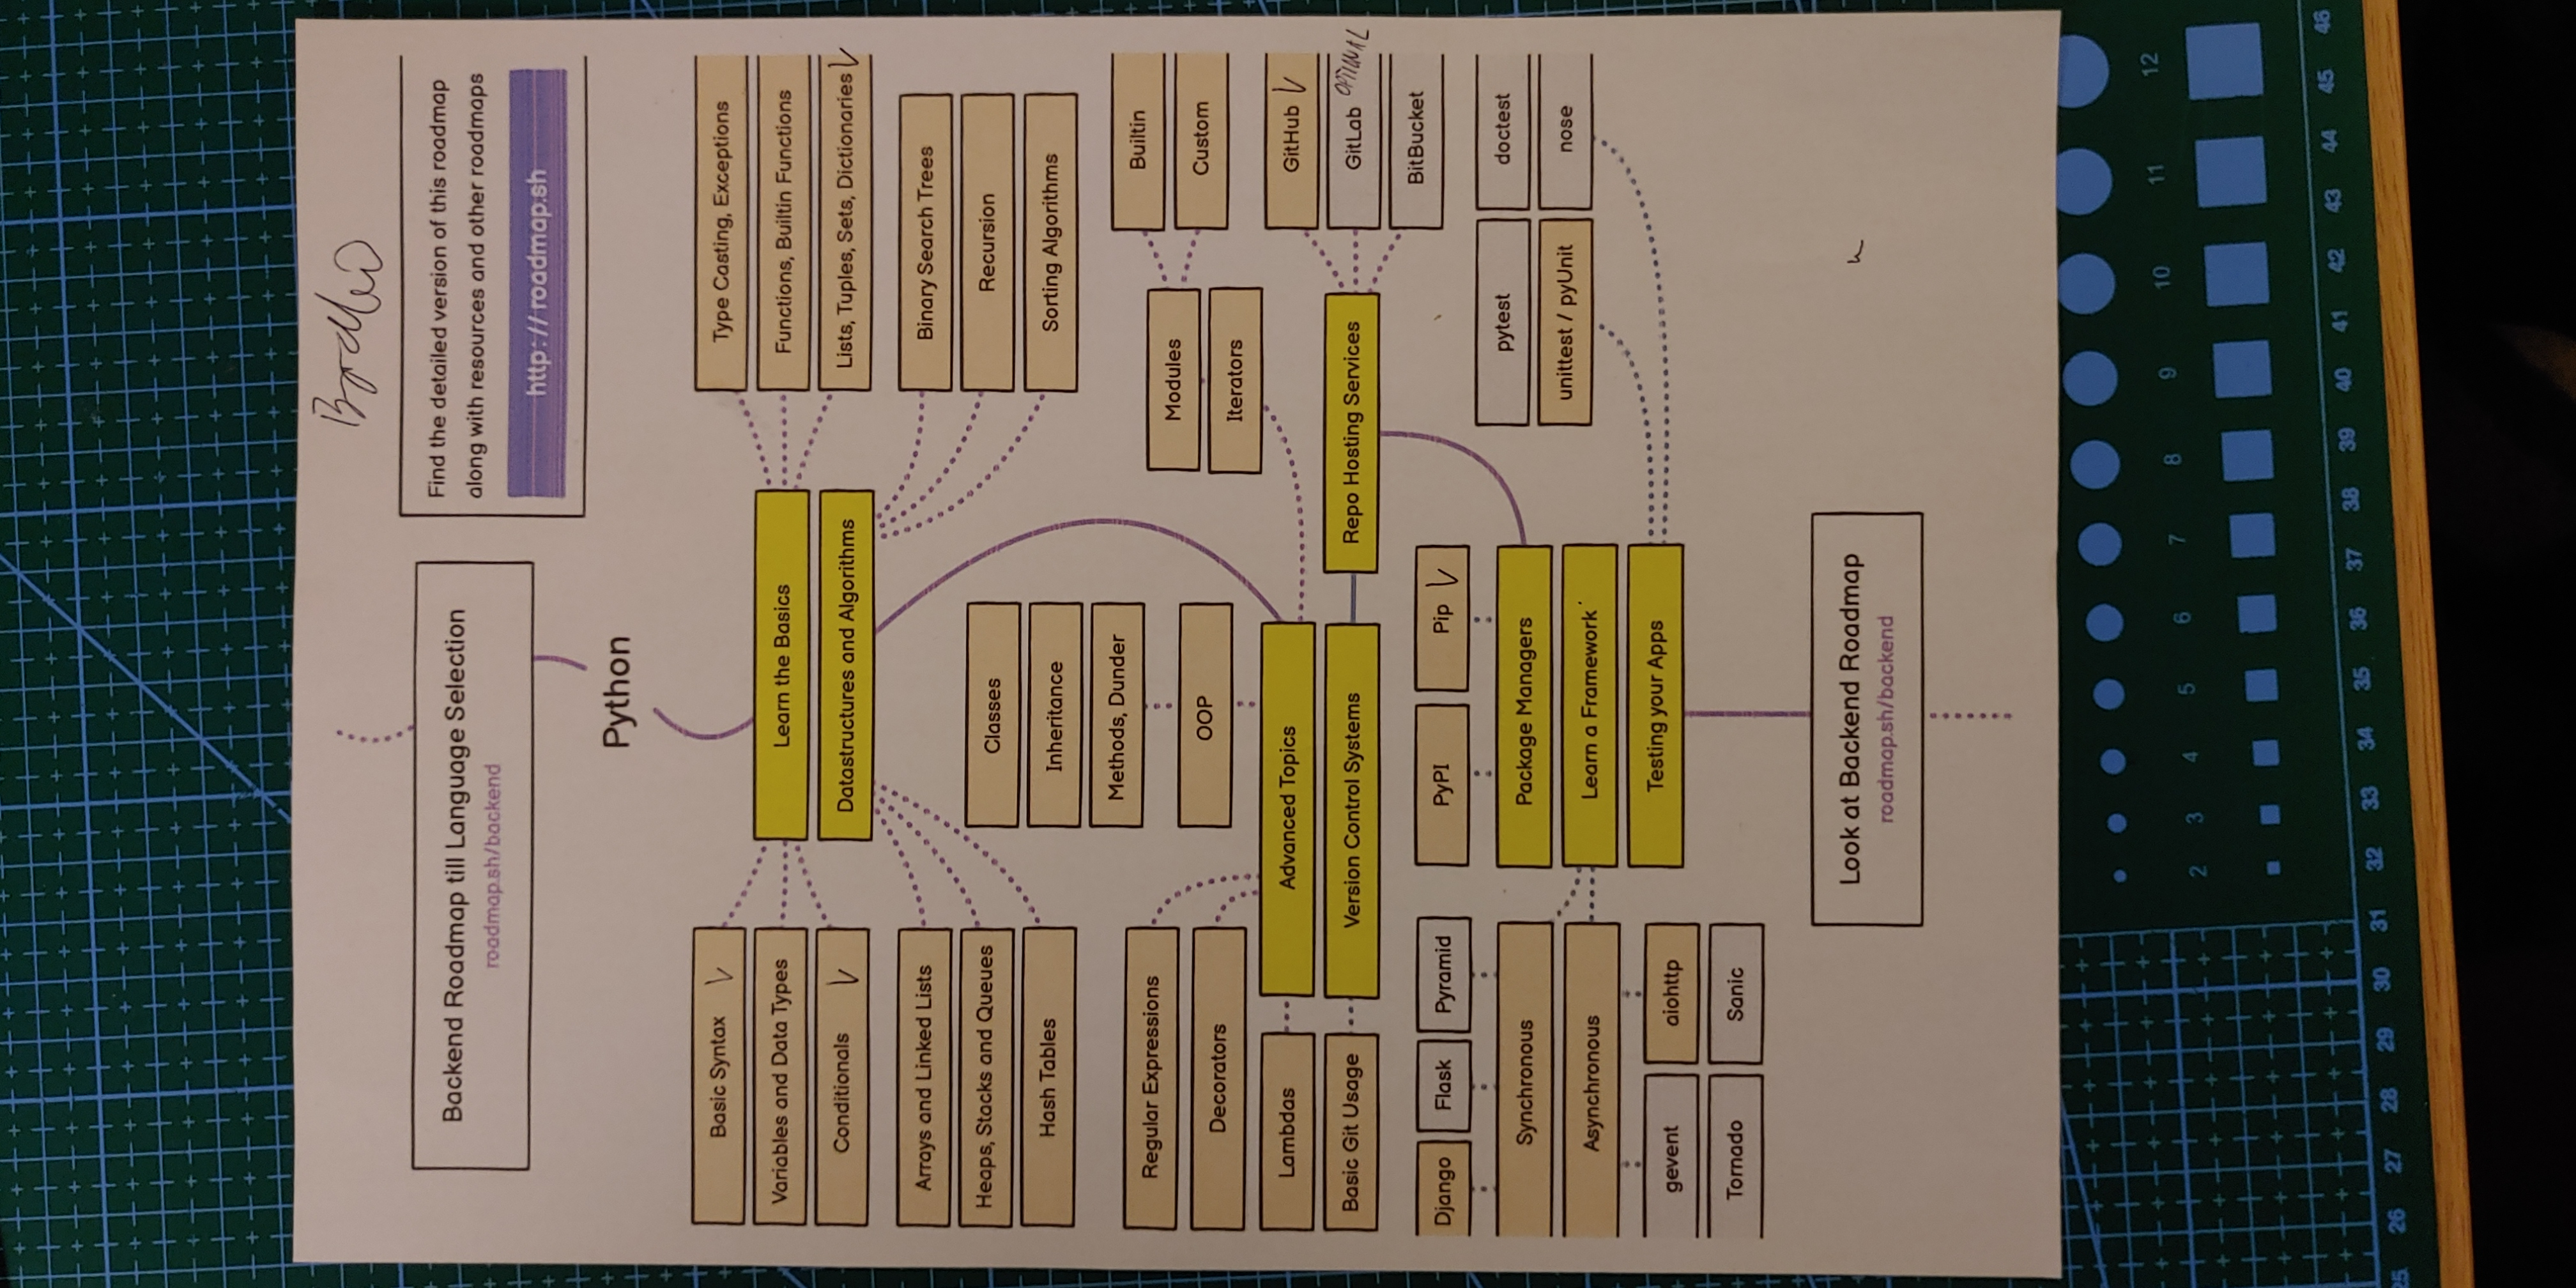
\includegraphics{orginal.png}
	}
\end{figure}
\begin{enumerate}
	\item Sprawdź czy skaner  działa poprawnie - Uruchomił się i poprawnie wykonał skan.
	\item Napisać program wykonujący skanowanie przy pomocy skanera płaskiego (WIA lub Twain - po ustaleniu z prowadzącym). Możliwości programu obejmują:
	      \begin{itemize}
		      \item skanowanie z wykorzystaniem  UI\\
		            UI występowało tylko podczas pracy z Windowsem okienko wyglądało następująco:
		            \begin{figure}[H]
			            \centering
			            \resizebox*{0.5\textwidth}{!}{
				            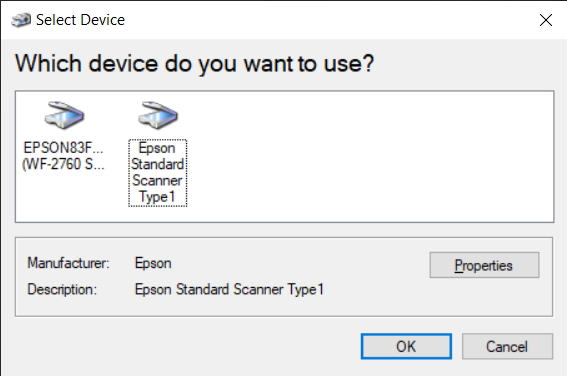
\includegraphics{detected_scanners.png}
			            }
		            \end{figure}
		            \begin{figure}[H]
			            \centering
			            \caption{Skan wynikowy}
			            \resizebox*{\textwidth}{!}{
				            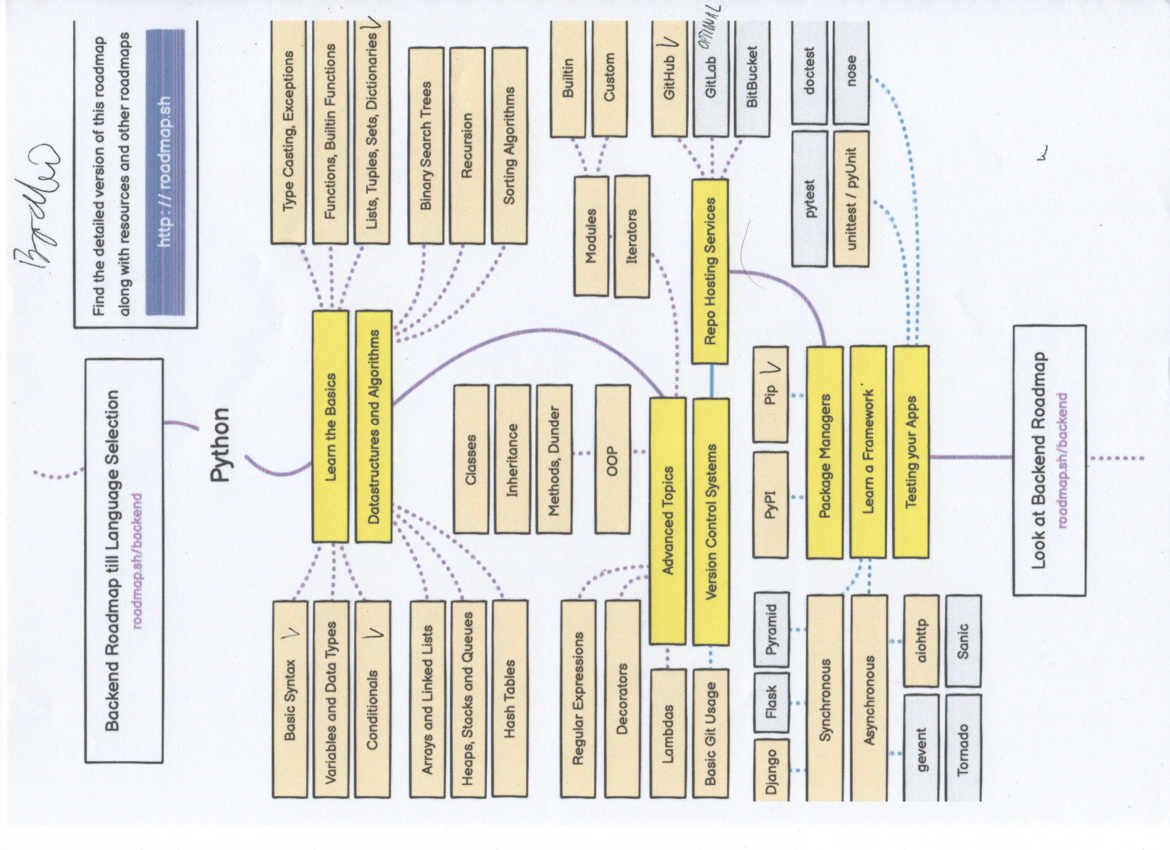
\includegraphics{wia-test.png}
			            }
		            \end{figure}
		            Kod za pomocą którego został wykonany skan.
		            \lstinputlisting{scan-windows.py}
		      \item skanowanie bez wykorzystania  UI\\
		            Tutaj pozostałe części zadania wykonywaliśmy na systemie operacyjnym Linux gdyż API było bardziej przejrzyste niż to z którego próbowaliśmy korzystać
		      \item wyświetlanie uzyskanego obrazu
		            \begin{figure}[H]
			            \centering
			            \resizebox*{0.5\textwidth}{!}{
				            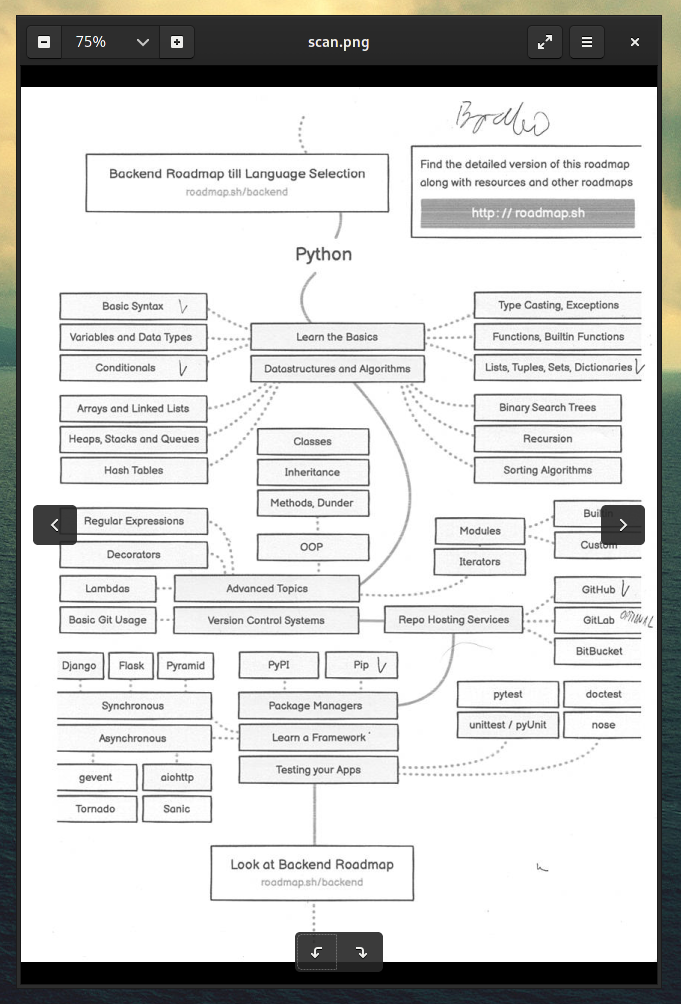
\includegraphics{editor_display.png}
			            }
		            \end{figure}
		      \item zmiana trybu skanowania (1-bitowy, skala szarości, RGB)
		            \begin{figure}[H]
			            \centering
			            \resizebox*{0.8\textwidth}{!}{
				            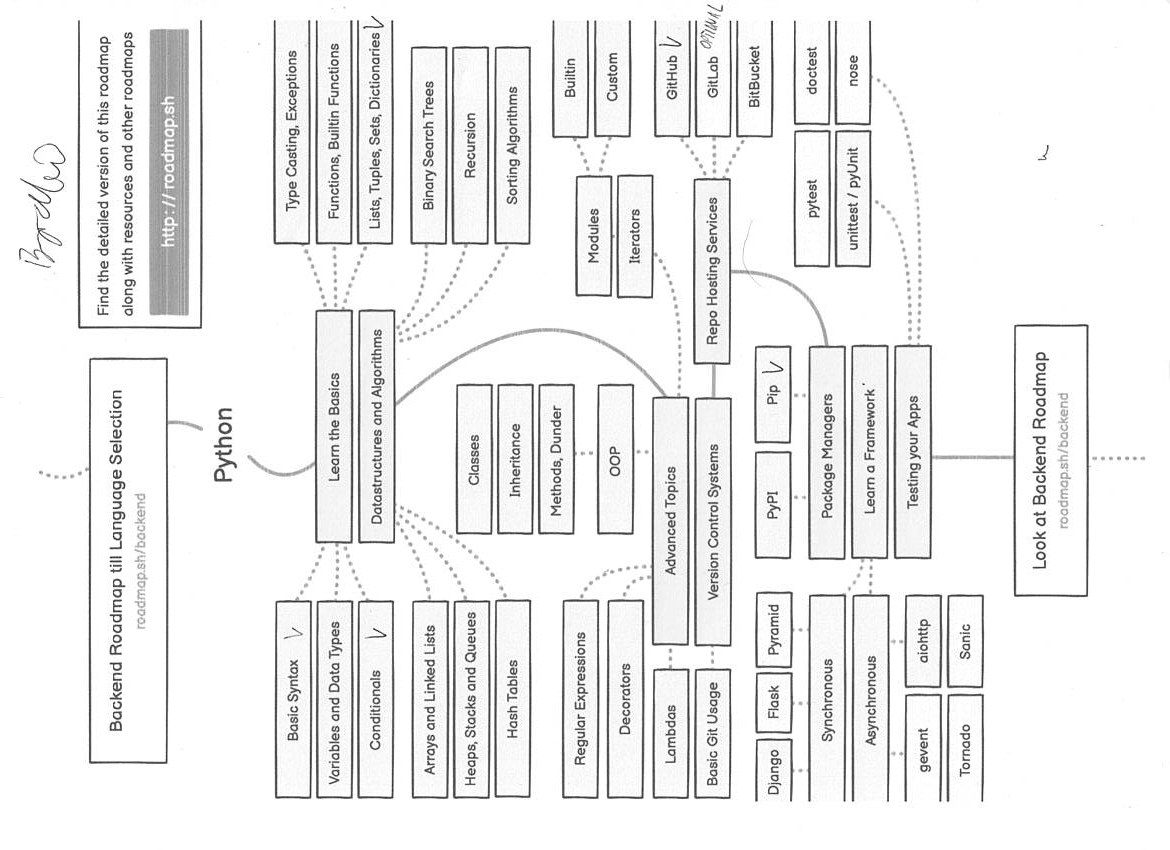
\includegraphics{grayscale.png}
			            }
		            \end{figure}
		      \item zmiana rozdzielczości skanera
		            \begin{figure}[H]
			            \centering
			            \resizebox*{\textwidth}{!}{
				            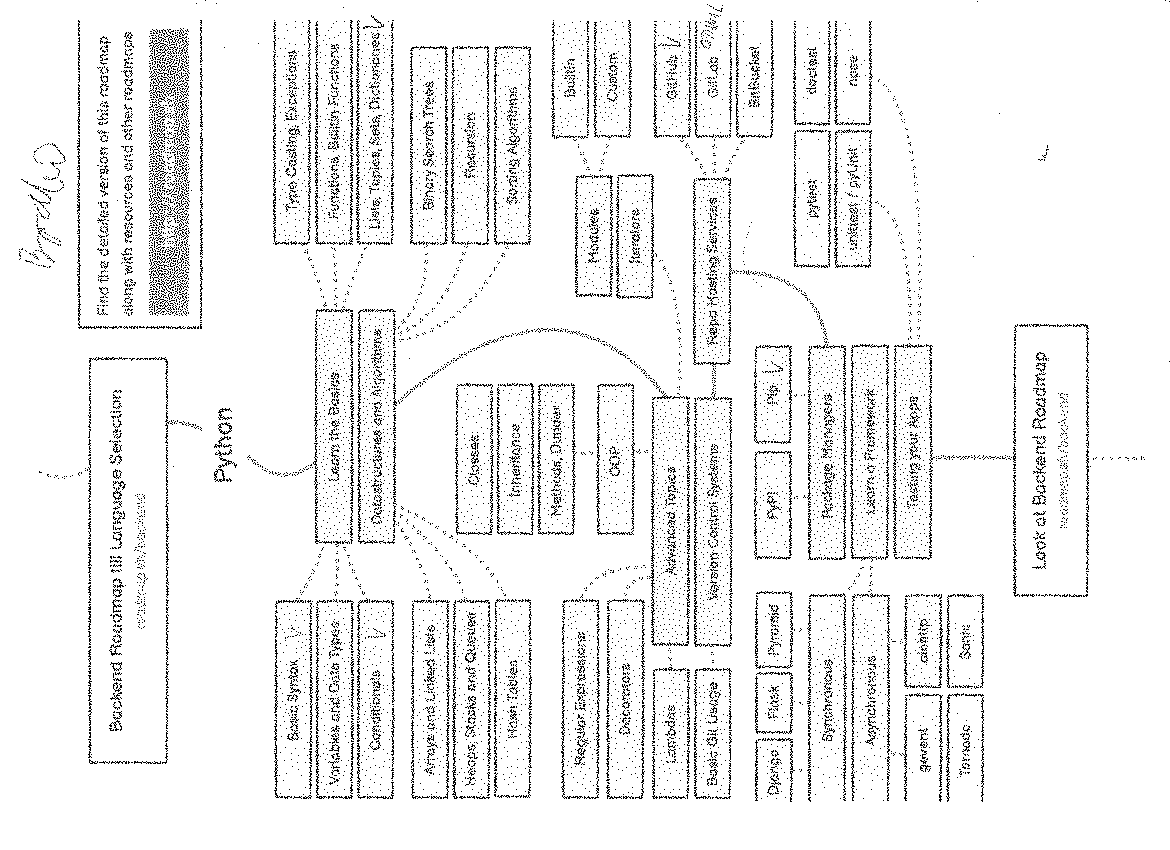
\includegraphics{bad_quality.png}
			            }
		            \end{figure}
	      \end{itemize}

	\item Rozszerzyć działanie programu:
	      \begin{itemize}
		      %   \item obsługa różnych trybów przesyłania danych
		      \item zapis skanowanych obrazów do plików graficznych - pliki są automatyczne zapisywane wraz z datą oraz godziną wykonania.

	      \end{itemize}
	\item kod programu wykorzystanym w systemie Linux
	      \lstinputlisting{skanuj.py}

\end{enumerate}
\section{Wnioski}
Windows ma bardzo okropne API dlatego w połowie wykonywania zadania przenieśliśmy się na system operacyjny Linux.
Znaleźliśmy w nim bibliotekę "Sane" która łączy się bezprzewodowo ze skanerem i może wykonywać wszystkie operacje wbudowane w skaner (wyświetlamy je po wpisaniu wybranych parametrów)

\end{document}